\documentclass[10pt,a4paper]{article}

%double si on veut une version prof et une version élève. simple si on veut une seule version.
\newcommand{\buildmode}{double}

\InputIfFileExists{version.tex}{}{}
% Version (définie par le script)
\providecommand{\version}{eleve}

\usepackage{feuilledistanciel}
\usepackage{schemaevolution}

%%%à modifier à chaque fois

\renewcommand{\niveau}{1STMG}
\renewcommand{\chapitre}{Révisions}
\renewcommand{\numchap}{1 à 3}
\renewcommand{\theme}{Travail en distanciel}

\begin{document}

\montitre{Révisions des premiers chapitres}

\textbf{Consignes de travail.} Traiter les sections dans l'ordre. Dans chaque section, commencer par les calculs de début de cours, sans calculatrice, puis lire attentivement le rappel de cours avant de traiter les exercices. Rédiger les réponses sur une copie, en justifiant et en faisant des phrases. Chercher d'abord seul, puis lire les indications seulement en cas de blocage. Comparer enfin avec la correction et reprendre ses erreurs d'une autre couleur.

\medskip

\begin{objectifs}
Lire graphiquement l'ensemble de définition, des images et des antécédents.\par\smallskip
Dresser un tableau de signes et un tableau de variations, et les traduire par des phrases.\par\smallskip
Compléter un tableau de valeurs et tracer une courbe.\par\smallskip
Calculer une proportion, un sous-effectif ou un effectif total.\par\smallskip
Lire et exploiter un tableau croisé : fréquences marginales et conditionnelles.\par\smallskip
Calculer un taux d'évolution, un coefficient multiplicateur, une valeur finale ou initiale.\par\smallskip
Calculer le taux d'évolution global d'évolutions successives.
\end{objectifs}

\prof{
    Fiche de révision des chapitres 1 (fonctions, généralités), 2 (proportions, tableaux croisés) et 3 (évolutions). Les calculs de début de cours reprennent les automatismes des semaines S1 à S3 de la progression. Pas de probabilités conditionnelles ici : on reste sur les fréquences. Durée indicative : 3 h d'exercices, puis 1 h de feuille blanche.
}

%%%%%%%%%%%%%%%%%%%%%%%%%%%%%%%%%%%%%%%%%%%%%%%%%%%%%%%%%%%%%%%%%%%%%%%%%%%%%
\section{Fonctions, généralités}

\begin{exo}[Calculs de début de cours]
Sans calculatrice.
\begin{enumerate}[leftmargin=*]
    \item Calculer :
    \begin{tasks}(3)
        \task \(-2+1\)
        \task \(1-2\)
        \task \(1+(-2)\)
        \task \(-5-3\)
        \task \(-4+(-6)\)
        \task \(7-(-2)\)
    \end{tasks}
    \item Écrire plus simplement en supprimant les symboles \og \(\times\) \fg lorsque c'est possible. 
    \begin{tasks}(4)
        \task \(1\times x\)
        \task \(-1\times x\)
        \task \(2\times x \times (3\times x+5)\)
        \task \(-4\times x-2\times(3\times 4+x) \)
    \end{tasks}
    \item Réduire les expressions suivantes :
    \begin{tasks}(2)
        \task \(2x+5-3x+1\)
        \task \(4x-7-x-2\)
        \task \(-x+3+2x-3\)
        \task \(5-2x+x-8\)
    \end{tasks}
\end{enumerate}
\end{exo}

\begin{indication}
    \begin{enumerate}
        \item On peut s'aider d'une droite graduée
        \item Un exemple est disponible dans l'annexe \ref{annexe-expr-mult} à la fin de la fiche.
        \item Voir l'annexe \ref{annexe-reduction} à la fin de la fiche.
    \end{enumerate}
\end{indication}

\begin{rappelcours}
Une fonction \(f\) associe à chaque nombre \(x\) de son \textbf{ensemble de définition} un unique nombre \(f(x)\). On note \(y=f(x)\) ou \(x\mapsto f(x)\).

\smallskip

Si \(f(a)=b\) : \(b\) est \textbf{l'image} de \(a\), et \(a\) est \textbf{un antécédent} de \(b\). Sur la courbe, l'image se lit sur l'axe des ordonnées et les antécédents sur l'axe des abscisses. Résoudre \(f(x)=k\), c'est trouver tous les antécédents de \(k\).

\smallskip

Le \textbf{tableau de signes} indique sur quels intervalles \(f(x)\) est positif (courbe au-dessus de l'axe des abscisses) ou négatif (courbe en dessous). Le signe ne peut changer qu'en un nombre où \(f(x)=0\).

\smallskip

Le \textbf{tableau de variations} indique sur quels intervalles \(f\) est croissante (la courbe monte) ou décroissante (la courbe descend), ainsi que les valeurs extrêmes : maximum et minimum.

\smallskip

\textbf{Exemple de traduction en phrase :} \og \(f\) est décroissante sur \([0\ ;\ 3]\) \fg{} ; \og le maximum de \(f\) sur \([0\ ;\ 8]\) est \(5\), atteint en \(x=6\) \fg{} ; \og \(f(x)\) est négatif pour \(x\) dans \([1\ ;\ 4]\) \fg{}.
\end{rappelcours}

\begin{exo}[Guidé]
Le graphique ci-dessous représente l'évolution de la température, en °C, à Saint-Denis au cours d'une journée d'hiver.

\begin{center}
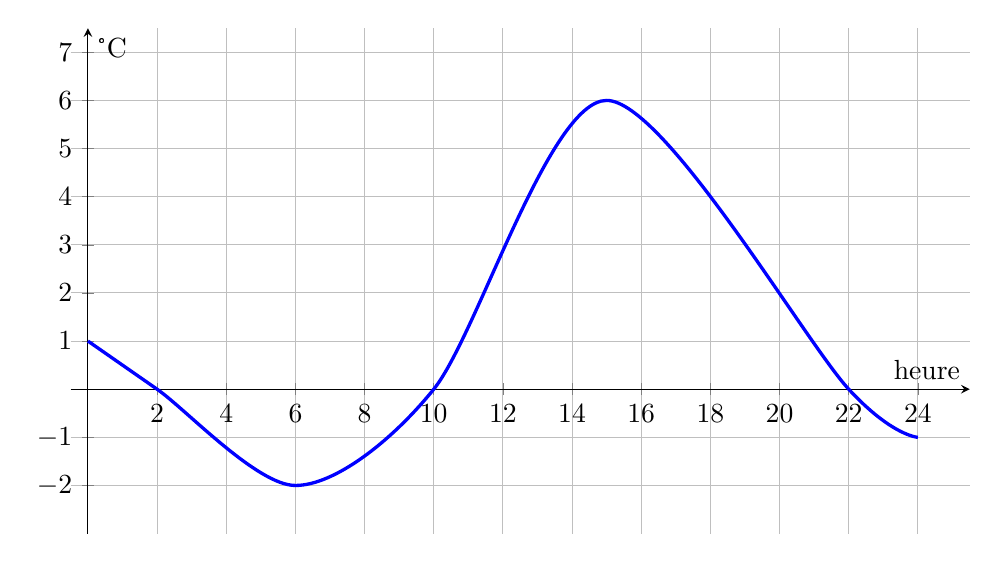
\begin{tikzpicture}
\begin{axis}[
    axis lines=middle,
    xmin=-0.5, xmax=25.5,
    ymin=-3, ymax=7.5,
    grid=major,
    xtick={0,2,...,24},
    ytick={-2,-1,...,7},
    xlabel={heure},
    ylabel={°C},
    width=13cm,
    height=8cm
]
\addplot[blue, very thick, smooth] coordinates {(0,1)(2,0)(6,-2)(10,0)(15,6)(22,0)(24,-1)};
\end{axis}
\end{tikzpicture}
\end{center}

\begin{enumerate}[leftmargin=*]
    \item Préciser sur quelle période les températures ont été relevées.
    \item Donner la température à 6 h, puis à 15 h.
    \item Donner les heures où la température était de \(0\)°C.
    \item Donner les plages horaires pendant lesquelles la température a augmenté.
    \item Donner les températures extrêmes de la journée, et les heures où elles ont été atteintes.
    \item On note \(f\) la fonction qui, à l'heure \(t\), associe la température \(f(t)\). Reformuler les réponses aux questions 1, 2 et 3 avec le vocabulaire des fonctions : ensemble de définition, image, antécédent.
    \item Dresser le tableau de signes de \(f\), puis le tableau de variations de \(f\).
    \item Traduire chacun des deux tableaux par une ou plusieurs phrases, dans le contexte de l'exercice.
\end{enumerate}

\begin{indication}
Pour le tableau de signes, repérer les heures où la courbe coupe l'axe des abscisses. Pour le tableau de variations, repérer les heures où la courbe change de sens.
\end{indication}

\checkpoint{le tableau de signes contient trois zéros et le tableau de variations comporte trois flèches.}
\end{exo}

\prof{
    Exercice 2 : même démarche que l'activité sur la température du chapitre 1, d'abord dans le contexte puis avec le vocabulaire des fonctions. Insister sur la verbalisation des tableaux.
}

\begin{exo}
On considère une fonction \(g\) dont la représentation graphique est donnée ci-dessous.

\begin{center}
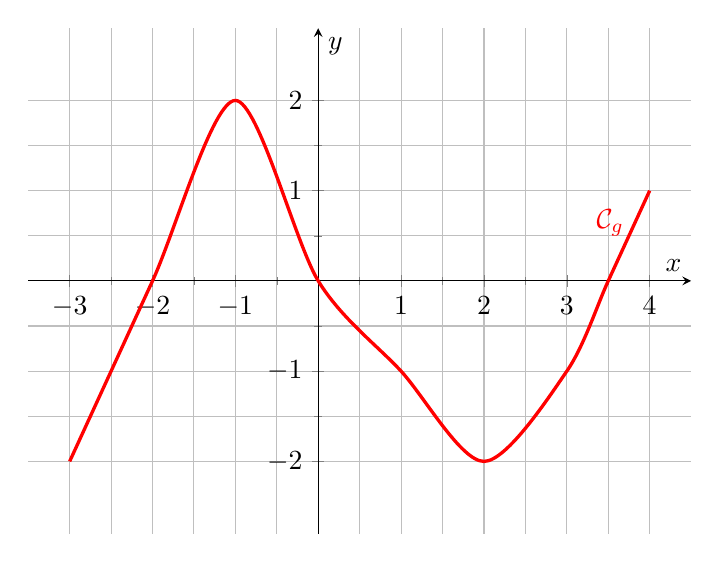
\begin{tikzpicture}
\begin{axis}[
    axis lines=middle,
    xmin=-3.5, xmax=4.5,
    ymin=-2.8, ymax=2.8,
    grid=both,
    minor tick num=1,
    xtick={-3,-2,...,4},
    ytick={-2,-1,...,2},
    xlabel={\(x\)},
    ylabel={\(y\)},
    width=10cm,
    height=8cm
]
\addplot[red, very thick, smooth] coordinates {(-3,-2)(-2,0)(-1,2)(0,0)(1,-1)(2,-2)(3,-1)(3.5,0)(4,1)}
node[pos=0.97, left] {\(\mathcal{C}_g\)};
\end{axis}
\end{tikzpicture}
\end{center}

\begin{enumerate}[leftmargin=*]
    \item Donner l'ensemble de définition de \(g\).
    \item Donner les images de \(-1\), de \(1\) et de \(4\) par \(g\).
    \item Donner les éventuels antécédents de \(2\), puis de \(0\).
    \item Résoudre graphiquement l'équation \(g(x)=-2\).
    \item Dresser le tableau de signes de \(g\) sur son ensemble de définition.
    \item Dresser le tableau de variations de \(g\) sur son ensemble de définition.
\end{enumerate}
\end{exo}

\begin{exo}
On considère la fonction \(h\) définie sur l'intervalle \([0\ ;\ 5]\) par \(h(x)=x^2-4x+3\).
\begin{enumerate}[leftmargin=*]
    \item Compléter le tableau de valeurs suivant.

    \begin{center}
    \renewcommand{\arraystretch}{1.5}
    \setlength{\tabcolsep}{0.3cm}
    \begin{tabular}{|c|c|c|c|c|c|c|}
        \hline
        \(x\) & \(0\) & \(1\) & \(2\) & \(3\) & \(4\) & \(5\) \\
        \hline
        \(h(x)\) & & & & & & \\
        \hline
    \end{tabular}
    \end{center}
    \item Placer les points du tableau dans le repère ci-dessous, puis tracer la courbe représentative de \(h\).

    \begin{center}
    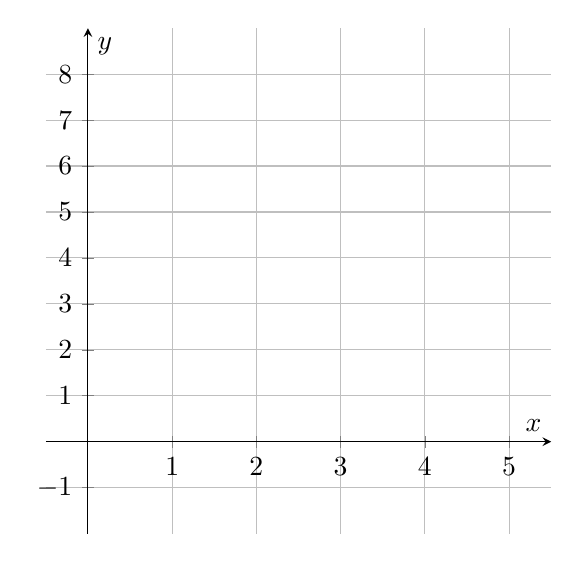
\begin{tikzpicture}
    \begin{axis}[
        axis lines=middle,
        xmin=-0.5, xmax=5.5,
        ymin=-2, ymax=9,
        grid=major,
        xtick={0,1,...,5},
        ytick={-1,0,...,8},
        xlabel={\(x\)},
        ylabel={\(y\)},
        width=8cm,
        height=8cm
    ]
    \end{axis}
    \end{tikzpicture}
    \end{center}
    \item Résoudre graphiquement l'équation \(h(x)=0\).
    \item Dresser le tableau de signes, puis le tableau de variations de \(h\) sur \([0\ ;\ 5]\).
\end{enumerate}
\end{exo}

\begin{exo}[][appro]
On considère une fonction \(k\) définie sur l'intervalle \([-4\ ;\ 6]\), dont on donne le tableau de variations et le tableau de signes.

\begin{center}
\begin{tikzpicture}
\tkzTabInit[lgt=1.1,espcl=1.6]{\(x\) /1, \(k\) /2}{\(-4\),\(-1\),\(3\),\(6\)}
\tkzTabVar{+/\(1\),-/\(-3\),+/\(5\),-/\(2\)}
\end{tikzpicture}
\qquad
\begin{tikzpicture}
\tkzTabInit[lgt=1.1,espcl=1.6]{\(x\) /1, \(k(x)\) /1}{\(-4\),\(-3\),\(1\),\(6\)}
\tkzTabLine{,+,z,-,z,+,}
\end{tikzpicture}
\end{center}

\begin{enumerate}[leftmargin=*]
    \item Traduire le tableau de variations par trois phrases, en utilisant les mots \og croissante \fg{}, \og décroissante \fg{}, \og maximum \fg{} et \og minimum \fg{}.
    \item Traduire le tableau de signes par deux phrases.
    \item Donner le nombre de solutions de l'équation \(k(x)=0\) sur \([-4\ ;\ 6]\).
    \item Tracer une courbe pouvant représenter la fonction \(k\).
\end{enumerate}
\end{exo}

\begin{exo}[][appro]
Une fonction \(m\) est définie sur \([-2\ ;\ 4]\) par le tableau de variations ci-dessous.

\begin{center}
\begin{tikzpicture}
\tkzTabInit[lgt=1.1,espcl=1.6]{\(x\) /1, \(m\) /2}{\(-2\),\(1\),\(4\)}
\tkzTabVar{+/\(3\),-/\(-1\),+/\(2\)}
\end{tikzpicture}
\end{center}

\begin{enumerate}[leftmargin=*]
    \item Tracer deux courbes différentes pouvant représenter la fonction \(m\).
    \item Expliquer pourquoi l'équation \(m(x)=0\) a exactement deux solutions.
    \item Peut-on donner la valeur exacte de ces solutions à l'aide du seul tableau de variations ? Peut-on tout de même donner l'allure du tableau de signes de \(m\) ? Justifier.
\end{enumerate}
\end{exo}

\prof{
    Exercice 6 : on attend un tableau de signes de la forme \(+\ 0\ -\ 0\ +\), avec des valeurs \(a\in\,]-2\ ;\ 1[\) et \(b\in\,]1\ ;\ 4[\) non connues. Bonne occasion de comparer les courbes tracées par les élèves.
}

%%%%%%%%%%%%%%%%%%%%%%%%%%%%%%%%%%%%%%%%%%%%%%%%%%%%%%%%%%%%%%%%%%%%%%%%%%%%%
\section{Proportions, pourcentages et tableaux croisés}

\begin{exo}[Calculs de début de cours]
Sans calculatrice, calculer et donner le résultat sous forme de fraction simplifiée.
\begin{tasks}(3)
    \task \(\dfrac{1}{2}+\dfrac{1}{4}\)
    \task \(\dfrac{2}{3}+\dfrac{1}{6}\)
    \task \(\dfrac{3}{5}-\dfrac{1}{10}\)
    \task \(1-\dfrac{2}{5}\)
    \task \(\dfrac{2}{3}\times\dfrac{3}{4}\)
    \task \(5\times\dfrac{2}{15}\)
\end{tasks}
\end{exo}

\begin{indication}
    Voir l'annexe \ref{annexe-fractions} pour avoir de l'aide sur les calculs de fractions.
\end{indication}


\begin{rappelcours}
\textbf{Proportion :} \(p=\dfrac{n}{N}\), où \(n\) est l'effectif de la sous-population et \(N\) l'effectif total. \quad \textbf{Sous-effectif :} \(n=p\times N\). \quad \textbf{Effectif total :} \(N=\dfrac{n}{p}\).

\smallskip

Un \textbf{tableau croisé} répartit une population selon deux critères.
\begin{itemize}
    \item Une \textbf{fréquence marginale} se calcule à partir d'un total (dernière ligne ou dernière colonne), divisé par l'effectif total.
    \item Une \textbf{fréquence conditionnelle} se calcule \textbf{à l'intérieur d'une sous-population} : on divise l'effectif d'une case par le total de sa ligne ou de sa colonne. Elle se repère souvent au mot \og parmi \fg{}.
\end{itemize}
\end{rappelcours}

\begin{exo}[Guidé]
Dans un lycée de \(400\) élèves, on a relevé le moyen de transport utilisé par chaque élève pour venir au lycée. Certaines cases du tableau ont été effacées.

\begin{center}
\renewcommand{\arraystretch}{1.5}
\begin{tabular}{|l|c|c|c|c|}
    \hline
    & \textbf{Transports en commun} & \textbf{Vélo} & \textbf{À pied} & \textbf{Total} \\
    \hline
    \textbf{Seconde} & \(80\) & \(20\) & & \(140\) \\
    \hline
    \textbf{Première} & \(70\) & & \(45\) & \(130\) \\
    \hline
    \textbf{Terminale} & & \(25\) & \(30\) & \(130\) \\
    \hline
    \textbf{Total} & & & & \(400\) \\
    \hline
\end{tabular}
\end{center}

\begin{enumerate}[leftmargin=*]
    \item Compléter le tableau.
    \item Calculer la proportion d'élèves de seconde dans le lycée. S'agit-il d'une fréquence marginale ou conditionnelle ?
    \item Calculer la proportion d'élèves qui viennent à vélo.
    \item Calculer la proportion d'élèves qui sont en terminale \textbf{et} qui viennent à pied.
    \item Parmi les élèves de première, calculer la proportion de ceux qui viennent à pied. S'agit-il d'une fréquence marginale ou conditionnelle ?
    \item Parmi les élèves qui viennent à vélo, calculer la proportion d'élèves de seconde.
\end{enumerate}
Donner les résultats sous forme décimale, arrondis au millième si nécessaire.

\begin{indication}
Le mot \og parmi \fg{} indique la sous-population de référence : c'est par son effectif que l'on divise. Pour la question 4, on divise par l'effectif total.
\end{indication}

\checkpoint{dans le tableau complété, la somme des totaux de la dernière ligne est bien égale à \(400\).}
\end{exo}

\begin{exo}
\begin{enumerate}[leftmargin=*]
    \item Un lycée compte \(1\,200\) élèves, dont \(15\,\%\) sont en série STMG. Calculer le nombre d'élèves en série STMG.
    \item Dans une entreprise de Seine-Saint-Denis, \(84\) salariés sont en télétravail, ce qui représente \(35\,\%\) des salariés. Calculer le nombre total de salariés.
    \item Dans une classe de \(35\) élèves, \(40\,\%\) sont des filles. Calculer le nombre de filles, puis le nombre de garçons.
\end{enumerate}
\end{exo}

\begin{indication}
    Une aide est disponible dans l'annexe \ref{annexe-proportions} pour les calculs de proportions.
\end{indication}

\begin{exo}
Un magasin a interrogé \(500\) clients sur leur moyen de paiement.

\begin{center}
\renewcommand{\arraystretch}{1.5}
\begin{tabular}{|l|c|c|c|c|}
    \hline
    & \textbf{Carte bancaire} & \textbf{Espèces} & \textbf{Téléphone} & \textbf{Total} \\
    \hline
    \textbf{Moins de 30 ans} & \(60\) & \(10\) & \(80\) & \(150\) \\
    \hline
    \textbf{30 ans et plus} & \(190\) & \(90\) & \(70\) & \(350\) \\
    \hline
    \textbf{Total} & \(250\) & \(100\) & \(150\) & \(500\) \\
    \hline
\end{tabular}
\end{center}

\begin{enumerate}[leftmargin=*]
    \item Calculer chacune des proportions suivantes, puis préciser s'il s'agit d'une fréquence marginale ou conditionnelle.
    \begin{enumerate}
        \item La proportion de clients qui paient par téléphone.
        \item Parmi les clients de moins de 30 ans, la proportion de ceux qui paient par téléphone.
        \item Parmi les clients qui paient en espèces, la proportion de clients de 30 ans et plus.
        \item La proportion de clients de moins de 30 ans.
    \end{enumerate}
    \item Calculer la proportion de clients qui ont moins de 30 ans \textbf{et} qui paient par carte bancaire.
    \item Vrai ou faux : \og Les clients de moins de 30 ans paient plus souvent par téléphone que les clients de 30 ans et plus. \fg{} Justifier à l'aide de fréquences.
\end{enumerate}
\end{exo}

\begin{exo}[QCM][bac]
Pour chaque question, une seule réponse est exacte. Justifier chaque réponse.
\begin{enumerate}[leftmargin=*]
    \item Le nombre \(\dfrac{3}{8}\) s'écrit en pourcentage :
    \begin{tasks}(4)
        \task \(0,375\,\%\)
        \task \(3,8\,\%\)
        \task \(37,5\,\%\)
        \task \(38\,\%\)
    \end{tasks}
    \item Un lycée compte \(800\) élèves, dont \(35\,\%\) sont demi-pensionnaires. Le nombre de demi-pensionnaires est :
    \begin{tasks}(4)
        \task \(35\)
        \task \(280\)
        \task \(520\)
        \task \(835\)
    \end{tasks}
    \item \(45\) personnes représentent \(30\,\%\) d'un groupe. Le groupe compte :
    \begin{tasks}(4)
        \task \(13,5\) personnes
        \task \(75\) personnes
        \task \(150\) personnes
        \task \(1\,500\) personnes
    \end{tasks}
    \item Dans le tableau de l'exercice 10, la proportion de clients de moins de 30 ans parmi ceux qui paient par carte bancaire est :
    \begin{tasks}(4)
        \task \(\dfrac{60}{500}\)
        \task \(\dfrac{60}{150}\)
        \task \(\dfrac{60}{250}\)
        \task \(\dfrac{250}{500}\)
    \end{tasks}
\end{enumerate}
\end{exo}

\prof{
    Exercice 11 : rappeler le format du QCM au bac et l'intérêt de justifier pour soi-même, même quand ce n'est pas demandé.
}

%%%%%%%%%%%%%%%%%%%%%%%%%%%%%%%%%%%%%%%%%%%%%%%%%%%%%%%%%%%%%%%%%%%%%%%%%%%%%
\section{Évolutions}

\begin{exo}[Calculs de début de cours]
Sans calculatrice.
\begin{enumerate}[leftmargin=*]
    \item Résoudre les équations suivantes.
    \begin{tasks}(4)
        \task \(2x+3=11\)
        \task \(5x-4=-19\)
        \task \(0,5x=6\)
        \task \(x+1,2=3\)
    \end{tasks}
    \item Écrire chaque nombre sous forme de fraction, la plus simple possible.
    \begin{tasks}(6)
        \task \(1,1\)
        \task \(0,9\)
        \task \(1,25\)
        \task \(0,75\)
        \task \(1,5\)
        \task \(0,8\)
    \end{tasks}
    \item Calculer \(1,1\times 1,2\) en écrivant d'abord \(1,1=\dfrac{11}{10}\) et \(1,2=\dfrac{12}{10}\).
\end{enumerate}
\end{exo}

\begin{indication}
    \begin{enumerate}
        \item Voir l'annexe \ref{annexe-equations} pour avoir de l'aide sur la résolution d'équations.
    \end{enumerate}
\end{indication}

\begin{rappelcours}
Une quantité passe d'une \textbf{valeur initiale} \(V_I\) à une \textbf{valeur finale} \(V_F\).
\begin{itemize}
    \item \textbf{Taux d'évolution :} \(t=\dfrac{V_F-V_I}{V_I}\). Il est positif pour une hausse, négatif pour une baisse. Multiplié par \(100\), il donne le pourcentage d'évolution.
    \item \textbf{Coefficient multiplicateur :} \(CM=1+t\). Une hausse de \(20\,\%\) correspond à \(CM=1,2\) ; une baisse de \(15\,\%\) à \(CM=0,85\).
    \item \(V_F=V_I\times CM\), \quad \(V_I=\dfrac{V_F}{CM}\), \quad \(CM=\dfrac{V_F}{V_I}\).
    \item \textbf{Évolutions successives :} le coefficient multiplicateur global est le \textbf{produit} des coefficients multiplicateurs. Les taux ne s'additionnent pas.
\end{itemize}
\schemaevolution{V_I}{V_F}{t}{\times CM}
\end{rappelcours}

\begin{exo}[Guidé]
Un sweat coûte \(60\) \euro. Pendant les soldes, son prix baisse de \(25\,\%\).
\begin{enumerate}[leftmargin=*]
    \item Recopier et compléter le schéma avec les données de l'énoncé.
    \schemaevolution{\dots}{\dots}{\dots}{\times \dots}
    \item Calculer le coefficient multiplicateur associé à cette baisse.
    \item En déduire le prix soldé du sweat.
    \item Après les soldes, le prix passe de ce prix soldé à \(54\) \euro. Calculer le taux d'évolution correspondant.
    \item Le prix est-il revenu à sa valeur initiale ? Calculer le coefficient multiplicateur global des deux évolutions, puis le taux d'évolution global.
\end{enumerate}

\begin{indication}
Pour une baisse de \(t\,\%\), le coefficient multiplicateur est \(1-t\). Pour la question 4, utiliser \(t=\dfrac{V_F-V_I}{V_I}\).
\end{indication}

\checkpoint{le prix soldé est un nombre entier d'euros, et l'évolution de la question 4 est une hausse.}
\end{exo}

\begin{exo}
Compléter le tableau suivant.

\medskip

\begin{center}
\renewcommand{\arraystretch}{1.5}
\begin{tabular}{|C{0.18\textwidth}|C{0.18\textwidth}|C{0.18\textwidth}|C{0.18\textwidth}|}
    \hline
    \textbf{Valeur initiale} & \textbf{Taux d'évolution} & \textbf{Coefficient multiplicateur} & \textbf{Valeur finale} \\ \hline
    \(40\) \euro & \(+15\,\%\) & \(\dots\) & \(\dots\) \\ \hline
    \(250\) \euro & \(-8\,\%\) & \(\dots\) & \(\dots\) \\ \hline
    \(120\) \euro & \(\dots\) & \(1,05\) & \(\dots\) \\ \hline
    \(80\) \euro & \(\dots\) & \(\dots\) & \(60\) \euro \\ \hline
    \(\dots\) & \(-40\,\%\) & \(\dots\) & \(36\) \euro \\ \hline
\end{tabular}
\end{center}
\end{exo}

\begin{exo}
\begin{enumerate}[leftmargin=*]
    \item Compléter les pointillés des deux schémas suivants.

    \schemaDeuxevolutions{500}{\dots}{\dots}{+20\,\%}{\dots}{-10\,\%}{\dots}{\times\dots}{\dots}

    \schemaDeuxevolutions{80}{\dots}{\dots}{-25\,\%}{\dots}{+25\,\%}{\dots}{\times\dots}{\dots}
    \item Une hausse de \(25\,\%\) compense-t-elle une baisse de \(25\,\%\) ? Justifier.
    \item Le loyer d'un local commercial a augmenté de \(3\,\%\) en 2025, puis de \(2\,\%\) en 2026. Calculer le coefficient multiplicateur global, puis le taux d'évolution global sur les deux années.
\end{enumerate}
\end{exo}

\begin{exo}[Vrai ou faux][appro]
Dire si chacune des affirmations suivantes est vraie ou fausse, en justifiant.
\begin{enumerate}[leftmargin=*]
    \item Une hausse de \(10\,\%\) suivie d'une hausse de \(10\,\%\) correspond à une hausse de \(20\,\%\).
    \item Une baisse de \(50\,\%\) suivie d'une hausse de \(100\,\%\) ramène à la valeur initiale.
    \item Augmenter un prix de \(30\,\%\) puis le diminuer de \(30\,\%\) revient à le diminuer de \(9\,\%\).
    \item Pour compenser une baisse de \(20\,\%\), il faut une hausse de \(20\,\%\).
\end{enumerate}
\end{exo}

\prof{
    Exercice 16, question 4 : chercher le coefficient \(CM\) tel que \(0,8\times CM=1\). Lien avec les équations des calculs de début de cours.
}

%%%%%%%%%%%%%%%%%%%%%%%%%%%%%%%%%%%%%%%%%%%%%%%%%%%%%%%%%%%%%%%%%%%%%%%%%%%%%
\section{Problèmes}

Les problèmes suivants mélangent les notions des trois sections précédentes.

\begin{exo}[Ventes de vélos]
Une entreprise de Seine-Saint-Denis vend des vélos électriques et des vélos classiques, en magasin et en ligne. Le tableau suivant donne ses ventes en 2025.

\begin{center}
\renewcommand{\arraystretch}{1.5}
\begin{tabular}{|l|c|c|c|}
    \hline
    & \textbf{En magasin} & \textbf{En ligne} & \textbf{Total} \\
    \hline
    \textbf{Vélos électriques} & \(180\) & \(120\) & \(300\) \\
    \hline
    \textbf{Vélos classiques} & \(270\) & \(130\) & \(400\) \\
    \hline
    \textbf{Total} & \(450\) & \(250\) & \(700\) \\
    \hline
\end{tabular}
\end{center}

\begin{enumerate}[leftmargin=*]
    \item Calculer la proportion de vélos vendus en ligne en 2025. Arrondir au millième.
    \item Parmi les vélos électriques, calculer la proportion de vélos vendus en ligne.
    \item En 2026, les ventes de vélos électriques augmentent de \(15\,\%\) et celles de vélos classiques baissent de \(10\,\%\). Calculer le nombre de vélos de chaque type vendus en 2026.
    \item Calculer le taux d'évolution du nombre total de vélos vendus entre 2025 et 2026. Arrondir à \(0,1\,\%\).
    \item Un employé affirme : \og Avec \(+15\,\%\) et \(-10\,\%\), les ventes totales ont augmenté de \(5\,\%\). \fg{} Expliquer pourquoi ce raisonnement est faux.
\end{enumerate}

\begin{indication}
À la question 3, appliquer chaque coefficient multiplicateur au total de sa ligne.
\end{indication}
\end{exo}

\begin{exo}[Population d'une commune]
Le graphique ci-dessous représente la population \(p(t)\) d'une commune de Seine-Saint-Denis, en milliers d'habitants, en fonction de l'année \(t\), entre 1990 et 2025.

\begin{center}
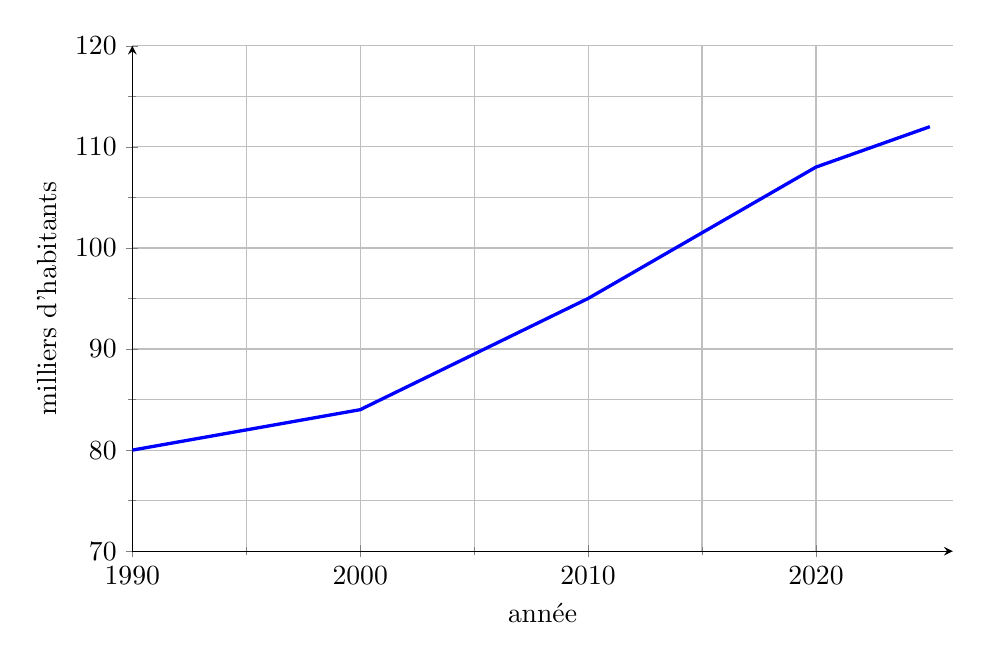
\begin{tikzpicture}
\begin{axis}[
    axis lines=left,
    xmin=1990, xmax=2026,
    ymin=70, ymax=120,
    grid=both,
    minor x tick num=1,
    minor y tick num=1,
    xtick={1990,2000,2010,2020},
    ytick={70,80,...,120},
    xticklabel style={/pgf/number format/1000 sep=},
    xlabel={année},
    ylabel={milliers d'habitants},
    width=12cm,
    height=8cm
]
\addplot[blue, very thick] coordinates {(1990,80)(2000,84)(2010,95)(2020,108)(2025,112)};
\end{axis}
\end{tikzpicture}
\end{center}

\begin{enumerate}[leftmargin=*]
    \item Donner l'ensemble de définition de la fonction \(p\), puis lire \(p(2000)\) et \(p(2020)\).
    \item Calculer le taux d'évolution de la population entre 2000 et 2020, en pourcentage arrondi à \(0,1\,\%\).
    \item Déterminer graphiquement l'année où la population a atteint \(100\,000\) habitants. Reformuler la réponse avec le mot \og antécédent \fg{}.
    \item Dresser le tableau de variations de \(p\). Traduire ce tableau par une phrase.
    \item La commune prévoit une hausse de \(2\,\%\) par an à partir de 2025. Calculer la population prévue en 2027.
\end{enumerate}
\end{exo}

\prof{
    Exercice 18, question 5 : deux hausses successives de \(2\,\%\), donc \(CM=1,02^2\). Ouverture possible vers les suites.
}

%%%%%%%%%%%%%%%%%%%%%%%%%%%%%%%%%%%%%%%%%%%%%%%%%%%%%%%%%%%%%%%%%%%%%%%%%%%%%
\section{Bilan}

Réaliser une très longue feuille blanche (1 h, soit \(3\times 20\) minutes) sur ce qui a été fait dans cette feuille. On rappelle que les objectifs de cette feuille étaient les suivants :

\medskip

Lire graphiquement l'ensemble de définition, des images et des antécédents.\par\smallskip
Dresser un tableau de signes et un tableau de variations, et les traduire par des phrases.\par\smallskip
Compléter un tableau de valeurs et tracer une courbe.\par\smallskip
Calculer une proportion, un sous-effectif ou un effectif total.\par\smallskip
Lire et exploiter un tableau croisé : fréquences marginales et conditionnelles.\par\smallskip
Calculer un taux d'évolution, un coefficient multiplicateur, une valeur finale ou initiale.\par\smallskip
Calculer le taux d'évolution global d'évolutions successives.

\prof{
    Feuille blanche : rappeler qu'elle est personnelle, sans cours ni fiche. Possibilité de la faire en trois temps de 20 minutes, en relisant la fiche entre deux temps.
}

\newpage

\begin{center}
    \Huge ANNEXES
\end{center}

\appendix

\section{Ecrire une expression en suivant les conventions} \label{annexe-expr-mult}

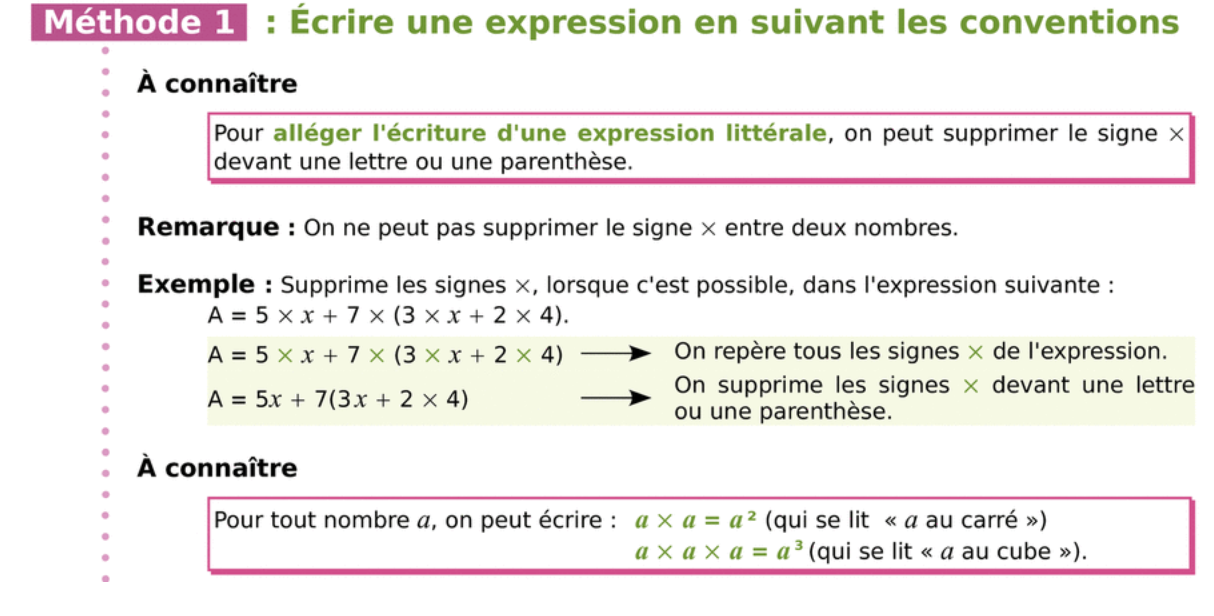
\includegraphics[width=0.9\textwidth]{annexe_sesamath_expr_mult.png}

\section{Réduire une expression développée} \label{annexe-reduction}

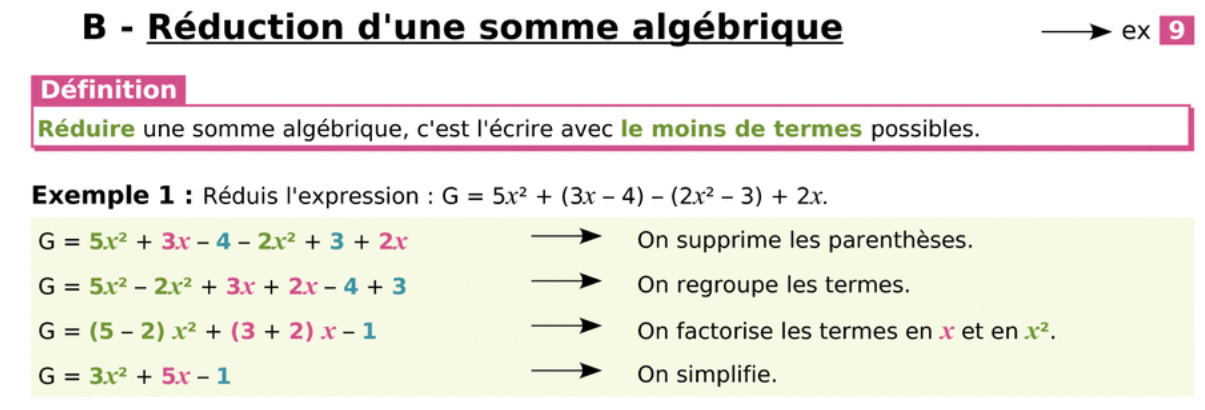
\includegraphics[width=0.9\textwidth]{annexe_sesamath_reduction.png}

\section{Calculer avec des fractions} \label{annexe-fractions}

\subsection{Simplifier une écriture fractionnaire}

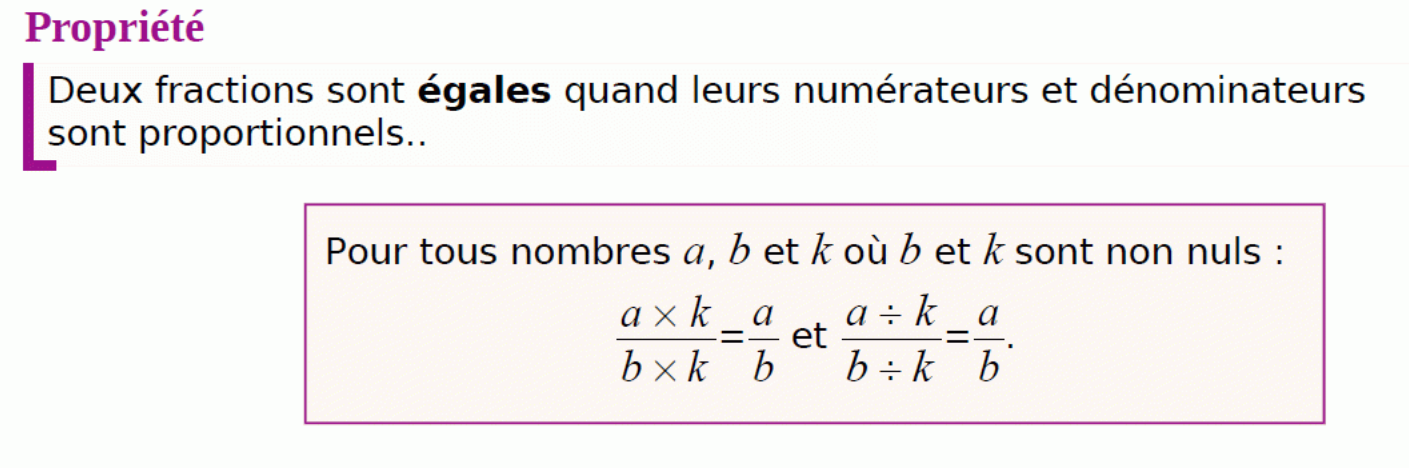
\includegraphics[width=0.9\textwidth]{annexe_sesamath_simpl_frac.png}

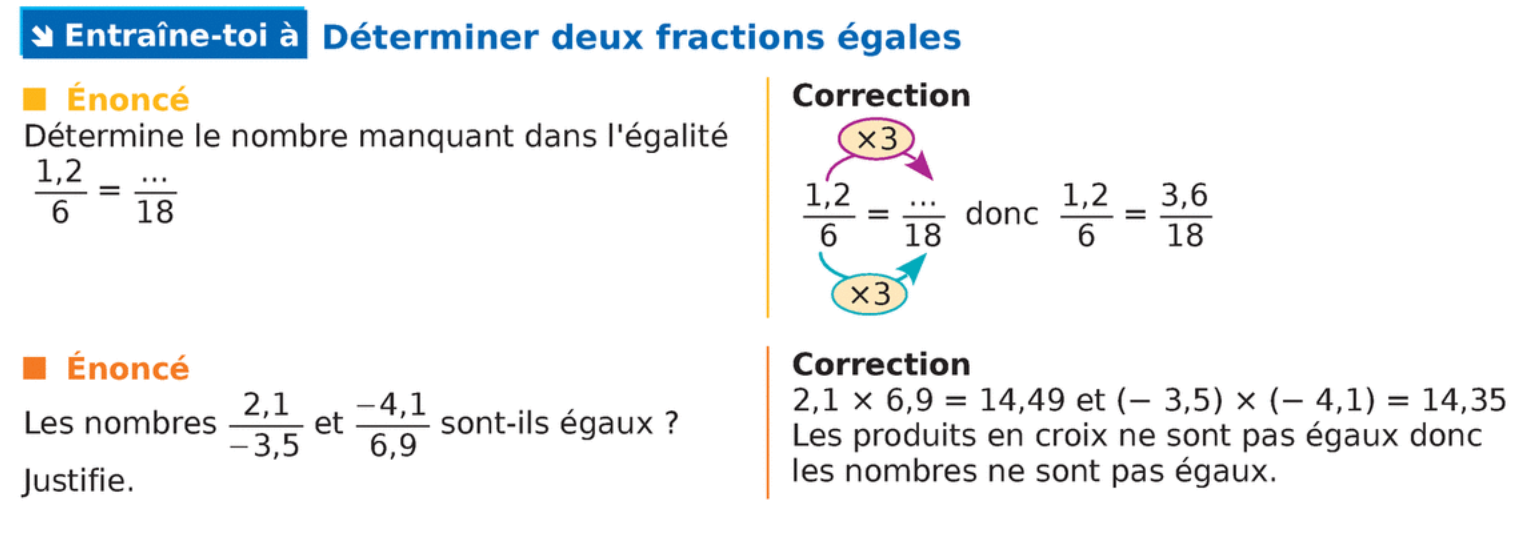
\includegraphics[width=0.9\textwidth]{annexe_sesamath_simpl_frac_exemple.png}

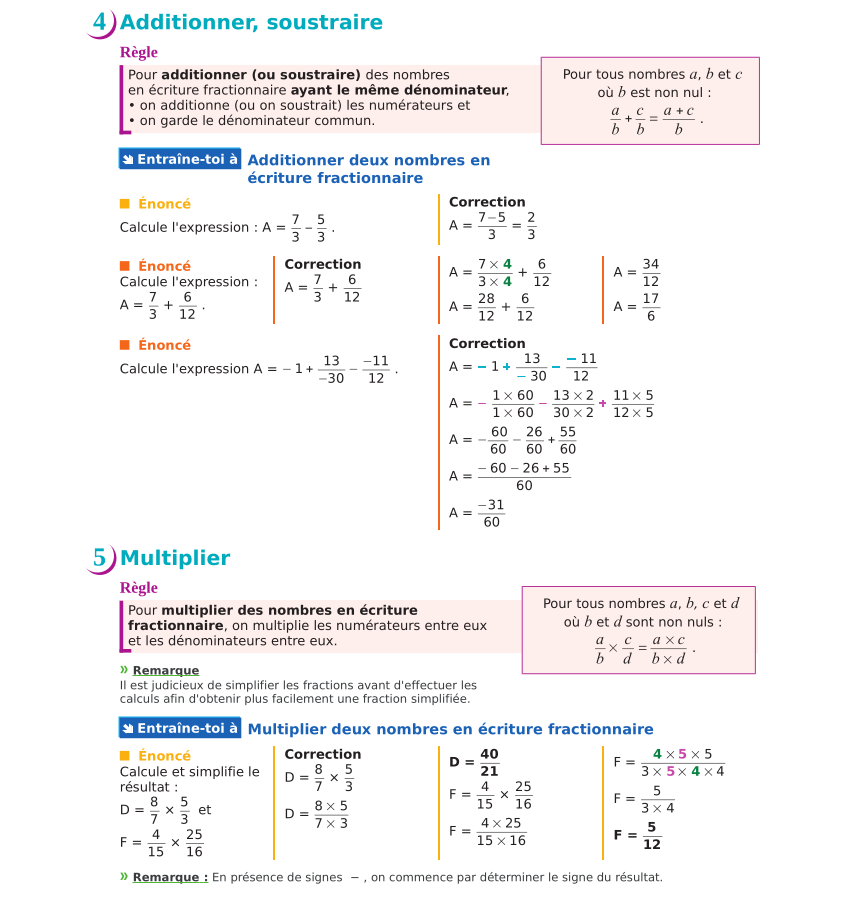
\includegraphics[width=0.9\textwidth]{annexe_sesamath_frac_operations.png}

\section{Calculer avec des proportions} \label{annexe-proportions}
\textbf{À connaitre : }
La proportion d'une valeur est le quotient : \(\dfrac{\text{effectif de la valeur}}{\text{effectif total}}\)

\textbf{Exemple : } Dans une classe de 30 élèves, 12 sont des filles. La proportion de filles est donc \(\dfrac{12}{30} = \dfrac{4}{10} = \dfrac{40}{10}\) Donc 40\% des élèves de la classe sont des filles.

\textbf{Remarque : }
On peut utiliser un tableau de proportionnalité :
\medbreak
\begin{tabular}{|c|c|c|c|}
    \hline 
    Effectif de la valeur & 12 & 4 & 40 \\
    \hline
    Effectif total & 30 & 10 & 100 \\
    \hline
\end{tabular}

\medbreak
\textbf{Méthode : }
On peut utiliser un tableau de proportionnalité pour retrouver un effectif de la valeur ou un effectif total. 

Exemples : Un lycée compte 1400 élèves, dont 15\% sont en série STMG. On cherche le nombre d'élèves en série STMG. \\
    
\begin{tabular}{|c|c|c|}
\hline
Effectif de la valeur & \tikzmarknode{A}{15} & \tikzmarknode{B}{210} \\
\hline
Effectif total & 100 & 1400 \\
\hline
\end{tabular}

\begin{tikzpicture}[remember picture, overlay]
\draw[->] ([yshift=5pt]A.north) to[bend left=20]
    node[above] {$\times 14$} ([yshift=5pt]B.north);
\end{tikzpicture}

Il y a 210 élèves en série STMG.

\section{Résoudre une équation} \label{annexe-equations}

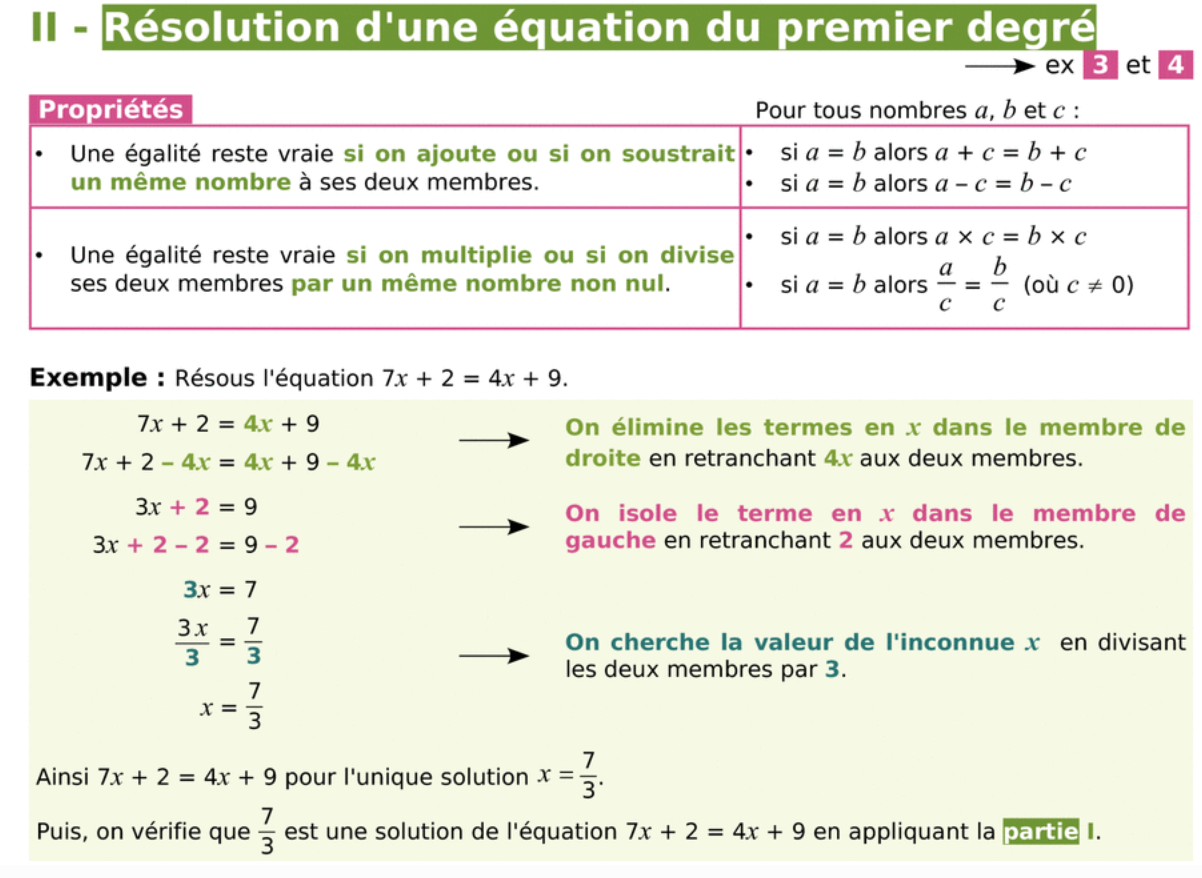
\includegraphics[width=0.9\textwidth]{annexe_sesamath_equations.png}
\end{document}
